\documentclass[10pt]{article}

\usepackage{amsfonts, amsthm, amsmath, fullpage, tikz, wrapfig, enumerate}

\newcommand{\card}[1]{\left| #1 \right|}
\newcommand{\nat}{\mathbb{N}}
\newcommand{\ints}{\mathbb{Z}}
\newcommand{\reals}{\mathbb{R}}
\newcommand{\chtitle}[1]{\noindent \vspace{5mm}\textbf{Chapter #1}\vspace{3mm}}
\newcommand{\images}{/home/gparker/classes/341/images}

\begin{document}
\begin{flushleft}
\textbf{\noindent
CS 341 Automata Theory \\
Geoffrey Parker - grp352\\
Homework 12 \\
Due: Tuesday, April 10}\\
\end{flushleft}
\noindent
This assignment covers Chapter 20.\\

\begin{enumerate}[1)]

% ---
% 1
% ---

\item
* Let $L_1, L_2, \ldots , L_k$ be a collection of languages over some alphabet $\Sigma$ such that:
\begin{itemize}
\item
For all $i \neq j$, $L_i \cap L_j = \emptyset$.
\item
$L_1 \cup L_2 \cup \dots \cup L_k = \Sigma ^*$.
\item
$\forall i$ ($L_i$ is in SD).
\end{itemize}
Prove that each of the languages $L_1$ through $L_k$ is in $D$.
\begin{proof}[Proof]
\end{proof}

%---
% 2
%---

\item
If $L_1$ and $L_3$ are in D and $L_1 \subseteq L_2 \subseteq L_3$, what can we say about whether $L_2$ is in D?
\begin{proof}[Answer]
Let $L_1$ be $\emptyset$ and $L_3$ be the language of all turing machines.  If $L_2$ is $\emptyset$, then it's decidable, if $L_2$ is $H$, then it's semidecidable but not decidable, and if $L_2$ is $\lnot H$ then it's not even semidecidable.  In all three cases $L_1 \subseteq L_2 \subseteq L_3$, so we can't say anything at all about $L_2$.
\end{proof}

% ---
% 3
% ---

\item
Let $M$ be a Turing machine that lexicographically enumerates the language $L$. Prove that there exists a Turing
machine $M'$ that decides $L^R$.
\begin{proof}[Proof]
Construct $M'$, a turing machine with input $w$.  $M'$ will use $M$ to start generating a lexicographic enumeration of $L$. If it encounters $w^R$, it will halt and return $true$.  If it encounters a string longer than $w$, it will halt and return $false$.  Thus $M'$ decides $L^R$.
\end{proof}


% ---
% 4
% ---

\item
Construct a standard one-tape Turing machine $M$ to enumerate the language $A^nB^n$. Assume that $M$ starts with
its tape equal to $\square$. Also assume the existence of the printing subroutine $P$, defined in Section 20.5.1.
\begin{proof}[Solution]
$PR_\square bL_\square a$ then loop.\\
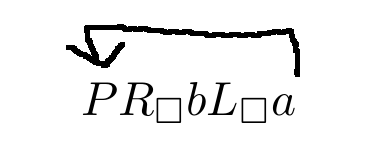
\includegraphics[scale=.3]{solution4.png}
\end{proof}

\pagebreak
% ---
% 5
% ---

\item
Recall the function $mix$, defined in Example 8.23. Neither the regular languages nor the context-free languages
are closed under $mix$. Are the decidable languages closed under $mix$? Prove your answer.
\begin{proof}[Answer]
Yes.
\end{proof}
\begin{proof}[Proof]
Let $L$ be a decidable language and $M$ be a machine that decides $L$.  Then we can construct $M'$, a machine that decides $mix(L)$ by first using the subroutine $X$ to mix the input string, then passing control to $M$ to decide if the string is in $L$ or not.\\

The subroutine $X$ works as follows:\\
\begin{enumerate}[1.]
\item
Find the midpoint of the input string.

\item
Move left to right over the second half of the string, overwriting it with blanks and copying it right to left onto tape 2.  This generates the reverse of the second half of the string on the second tape.

\item
Copy the contents of tape two back onto the end of the remaining string on tape 1.
\end{enumerate}
\end{proof}


% ---
% 6
% ---

\item
Let $\Sigma = \{a, b\}$. Consider the set of all languages over $\Sigma$ that contain only even length strings.
\begin{enumerate}[a)]
%a
\item
How many such languages are there?
\begin{proof}[Answer]
Uncountably infinitely many.  It's the powerset of even length strings over $\Sigma$.
\end{proof}


%b
\item
How many of them are semidecidable?
\begin{proof}[Answer]
Countably infinitely many.  Shown in theorem 20.3 in the book.
\end{proof}
\end{enumerate}
\end{enumerate}
\end{document}
